% camera ready
\section{The Metagame and Our Approach}

\subsection{The Metagame}
\label{subsection_metagame}

Currently, there are two popular high performing agents that people have shared during the competition. They are PubHRL \cite{notebook_pubhrl} and AlphaGeese \cite{notebook_alphageese_baseline}.

\begin{figure}[h]
\centering
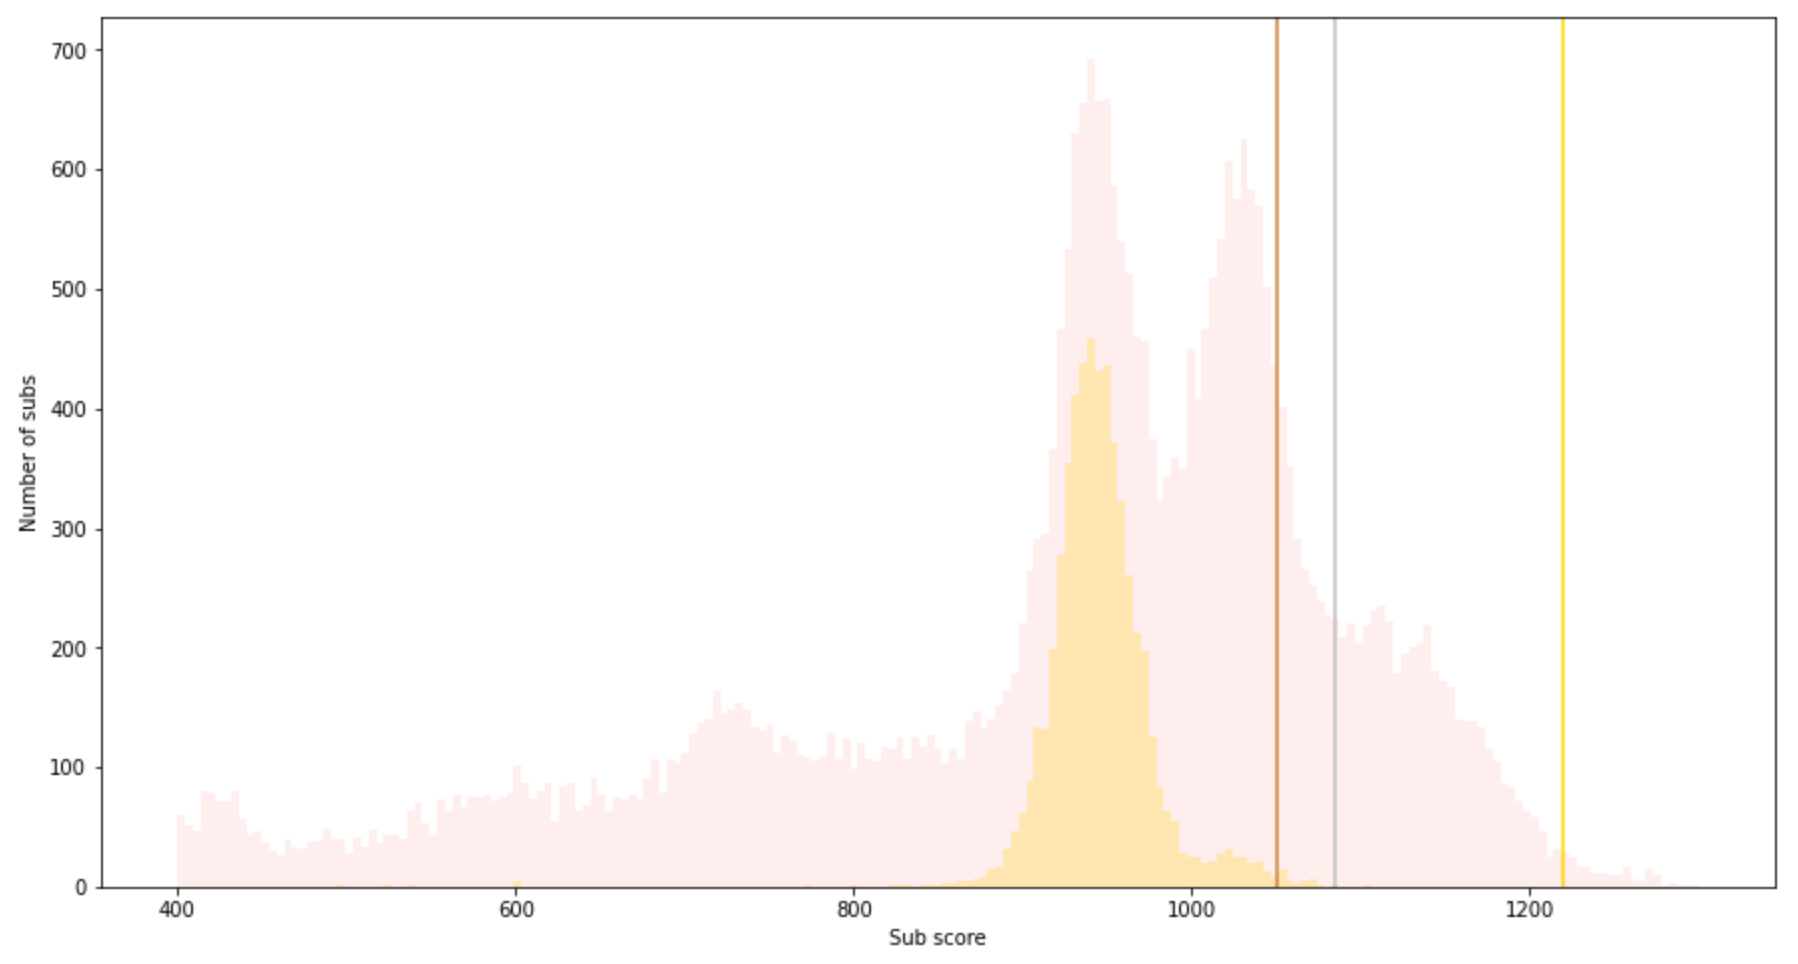
\includegraphics[width=\textwidth]{images/metagame.png}
\caption{Distribution of Scores of Submitted Agents}
\label{figure_metagame}
\end{figure}

Figure \ref{figure_metagame}, which is produced by a top participating team \cite{comment_agent_score_distribution}, shows the distribution of scores of submitted agents at the close of the submissions. The vertical lines show the required team rating to get a Kaggle Bronze, Silver or Gold medal.

The first peak is heavily contributed by PubHRL \cite{notebook_pubhrl}. PubHRL was published in February. It has been analysed that the agents shaded in yellow in Figure \ref{figure_metagame} makes moves exactly suggested by PubHRL, and the agents make up to 17.5\% of the submissions \cite{comment_agent_score_distribution}. PubHRL is a neural network model that suggest which move to take. We will elaborate on PubHRL in Section \ref{section_nn_model}.

The second peak is suspected to be heavily contributed by AlphaGeese \cite{notebook_alphageese_baseline}. AlphaGeese was published in April. AlphaGeese model uses PubHRL model inferences but it improves the performance by adding Monte Carlo Tree Search (MCTS) algorithm on top of it. This approach is similar to AlphaGo \cite{paper_alphago}, and we will elaborate this in Section \ref{section_mcts}

\subsection{Our Approach}
\label{subsection_approach}

When we entered the competition, we have decided to improve on the best-performing approach that has been published, which is AlphaGeese. There are two aspects we can improve on AlphaGeese. One aspect is to improve the underlying neural network model in terms of performance or time, which we will explore in Section \ref{section_nn_model}. The neural network model can be improved by changing the model architecture, which we will describe in Subsection \ref{subsection_alt_model_arch_hyper_param} or changing agents it is being trained against, which we will describe in Subsection \ref{subsection_training_against_different_agents}. The other aspect is to improve how Monte Carlo Tree Search is done, which we will explore in Section \ref{section_mcts}.

Then in Section \ref{section_discussion}, we describe and analyse the results. We will also show how to set up a GUI to play against specified agents in Section \ref{section_gui}.

% Explanation of the rule-based agents? (to write?)
% The strategy of Risk Adverse Greedy Goose.


